\chapter{Desenvolvimento}

\section{Introdução}

Neste capitulo serão apresentadas as etapas e os detalhes de desenvolvimento do sistema. No primeiro momento foram levantados os requisitos do sistema e identificados como funcionais e não funcionais. 
Após identificado os requisitos, deu-se inicio a modelagem dos diagramas utilizando a Linguagem de Modelagem Unificada (UML) cujo objetivo é representar de maneira gráfica as funcionalidades do sistema e as interações entre estas funcionalidades com os usuários. 


\section{Visão geral do trabalho}

O processo de desenvolvimento deste sistema foi estruturado baseado nas melhores práticas de engenharia de software. Para o sistema alcançar os objetivos deve: cadastrar de fornecedores, cadastrar de produtos, cadastrar clientes e manter orçamentos. 

\section{Requisitos}

O levantamento de requisitos é o primeiro passo para o desenvolvimento de software. Os requisitos são de extrema importância, pois refletem as necessidades do cliente. Neste processo devem-se identificar os requisitos, classificá-los em funcionais e não-funcionais, além de definir seu nível de prioridade para o sistema. A seguir, alguns requisitos que o sistema deve atender.

\subsection{Requisitos funcionais}
Um requisito funcional define uma função que um sistema deve executar. Logo, representa uma tarefa ou serviço que o sistema deve fazer. Os requisitos estão contidos no Anexo A deste documento na Tabela \ref{tab:rf01} a \ref{tab:rf19}


\subsection{Requisitos não funcionais}

Os requisitos não funcionais estão diretamente relacionados com as propriedades que o sistema todo ou de partes do sistema devem apresentar e estão contidos no Anexo B deste documento na Tabela \ref{tab:rnf01} a \ref{tab:rnf04}


\section{Diagramas UML}

A UML define uma série de diagramas que nos ajudam na tarefa de modelar e documentar o sistema orientado a objetos no ato de desenvolvimento. Atualmente, a UML está na versão 2.2 e possui 14 tipos de diagramas que nos ajudam a prevenir problemas encontrados em um sistema orientado a objetos. 

\subsection{Diagrama de casos de uso}
O diagrama de caso de uso apresenta de forma visual os principais requisitos do sistema e sua interação com cada ator (usuário).

\begin{figure}[htp]
\centering
\caption{Diagrama de casos de uso}
\label{fig:Casodeuso}
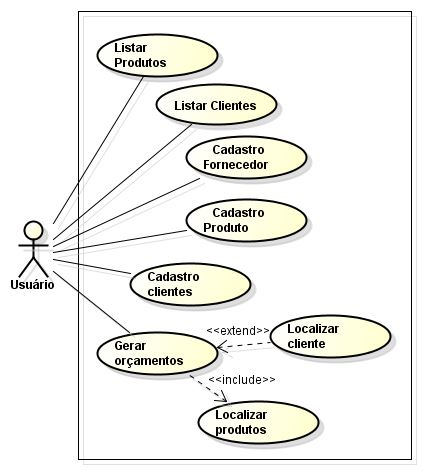
\includegraphics[width=13cm]{imagens/diagramas/Caso-de-uso-}
\fonte{Autor próprio.}
\end{figure}

\subsection{Diagrama de atividade}

O diagrama de atividade representa graficamente os fluxos de uma atividade para outra. Neste diagrama são representados os pontos de início e fim de uma atividade, as ações que são realizadas durante o processo, além das decisões que são tomadas durante o fluxo de execução. Os diagramas de atividade do sistema estão localizados no anexo D deste documento.

\subsection{Diagrama de classes}


O diagrama de classes é um dos principais diagramas da UML. Seu objetivo é fornecedor ao desenvolvedor uma visão ampla dos pacotes de classes, bem como de seus métodos e variáveis. Segundo Guedes \cite{guedes2018uml}, o diagrama de classes serve ainda como base para a construção da maioria dos outros diagramas da UML.
O anexo C apresenta o diagrama de classes do sistema.
Na seção 4.6 deste capítulo, trataremos com mais detalhes as classes deste diagrama.


\subsection{Diagrama de sequência}

O diagrama de sequência é utilizado para representar a comunicação entre os objetos do sistema em determinado cenário. Baseia-se no diagrama de caso de uso sendo amparado pelo diagrama de classes. 
Segundo Guedes \cite{guedes2018uml}, um diagrama de sequência costuma identificar o evento gerador do processo, bem como o ator responsável pelo esse evento, e determina como o processo deve progredir e ser concluído. O anexo E deste documento trás os diagramas de sequência do sistema.




\subsection{Modelo de entidade-relacionamento}
Um banco de dados consiste em um conjunto de tabelas que armazenam dados de forma organizada.
Em um banco de dados relacional, são estabelecidos os relacionamentos entre as tabelas através de chaves primárias e chaves estrangeiras. 
Uma das vantagens em se utilizar o \textit{framework} Hibernate é o fato destas relações serem realizadas de maneira automática, através do mapeamento das entidades.
Utilizando a ferramenta MySQL Workbench é possível visualizar as relações entre as tabelas de maneira gráfica através do Diagrama de esquemas. O MER está disponível no anexo F deste documento,
Já o código para geração do banco de dados pode ser encontrado no anexo F deste documento.


\section{Codificação do sistema}

    \subsection{Organização das classes}
        Organizar as classes é uma boa prática de programação que  evita duplicidades e as mantém mais organizadas permitindo sua localização de forma mais eficiente. 
        Em Java as classes são organizadas em pacotes que são diretórios criados na raiz do projeto.  
        A organização das classes em pacotes também serve como indicação para o compilador Java para encontrar o arquivo que contém o código da classe \cite{ricarte2001programaccao}. 
        Neste projeto, os pacotes foram nomeados utilizando a seguinte sintaxe: br.com.softFlor.NOME-DO-PACOTE.

    
    \subsubsection{Package: br.com.softflor.conexao}
        Pacote destinado a classe responsável pela conexão com o Banco de dados. Neste pacote está contido a classe 'ConectaBD' responsável por abrir e fechar conexões com o banco de dados através dos métodos getEntityManager() e FechaConexao().
        
    \subsubsection{Package: br.com.softflor.dao}
    Neste pacote estão inseridos as classes DAO do sistema. Em geral, estas classes são responsáveis por trocar informações com o banco de dados e fornecer operações de CRUD e de pesquisas. 
    Neste pacote esta contido a classe GenericDAO responsável por realizar as tarefas comuns á todos os modelos. Esta classe recebe como parâmetro qualquer objeto que implementa a interface 'EntidadeBase'. Além disso, acessa através de herança os atributos e métodos da classe ConectaBD.
    Como esta classe é responsável por todas as tarefas de CRUD do sistema, as classes DAO individuais como, por exemplo, ClienteDAO e ProdutoDAO serão responsáveis por realizar consultas personalizadas no banco de dados.
     
    \subsubsection{Package: br.com.softflor.dao.tableModel}
        O Pacote tableModel é um subpacote de DAO. Neste pacote estão as classes que servem de modelo para as tabelas do sistema, sobretudo, as tabelas responsáveis por exibir as listas de produtos, clientes e fornecedores, além da tabela de listagem de produtos inseridos no orçamento.
        
    \subsubsection{Package: br.com.softflor.entidades}  
    O pacote de classes entidade contém as classes que servirão de modelo para os objetos criados. Em cada modelo deste pacote também estão contidas as anotações responsáveis por realizar o mapeamento das entidades que serão utilizadas pelo \textit{framework} Hibernate.
    
    \subsubsection{Package: br.com.softflor.views}  
     Neste pacote estão contidas todas as classes que tratam das interfaces gráficas do sistema. 
    
    \subsection{Hibernate}
    O Hibernate é responsável por todas as persistências de dados da aplicação, utilizando para tal o conceito de mapeamento de objeto-relacional (ORM). Este mapeamento é realizado em tempo de execução pelo \textit{framework} através de anotações inseridas nas classes do projeto. 
    No primeiro momento, foi necessário instalar todos os \textit{jars} necessários para o correto funcionamento do Hibernate. Após isso foi realizado a configuração do Hibernate utilizando o persistence.xml que por padrão, esta localizado na pasta META-INF da \textit{classpath} do sistema. 
    
   Após realizar estas configurações é necessário envia-las para o Hibernate, para isso é criado uma um objeto da classe \textit{EntityManagerFactory }passando o arquivo de configuração. Após obter o \textit{factory} poderemos estanciar um objeto \textit{EntityManager}, conforme a classe ConectaBD abaixo:
   
   
 \begin{figure}[htp]
\centering
\caption{Código - Conexão com banco de dados}
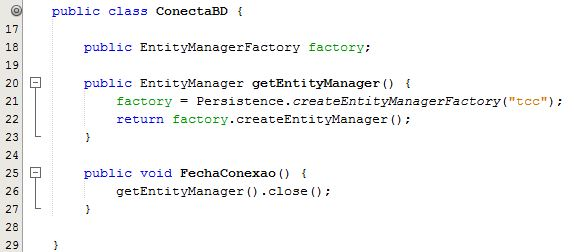
\includegraphics[width=15cm]{imagens/codigo/ConectaBD}
\fonte{Autor próprio}
\label{fig:conectaBD}
\end{figure}
   
   
    O Hibernate fornece como opções de mapeamento, modelos de objeto desenvolvidos com arquivos XML ou através de anotações no código fonte das classes de modelo. Neste projeto foi utilizado o método de anotações. A Tabela \ref{tab:anotacoes} mostra as principais anotações utilizadas.

\begin{table}[H]
\caption{Lista de anotações}
\label{tab:anotacoes}
\begin{tabular}{ll}
\hline
\multicolumn{2}{c}{Anotações utilizadas}                                        \\ \hline
@Entity         & Indica para que classe é uma entidade no banco de dados         \\ \hline
@Id             & Define o atributo como um Id                                    \\ \hline
@GeneratedValue & Define uma estratégia de geração de valor para o atributo       \\ \hline
@OneToOne       & Estabelece uma relação um para um com outra entidade            \\ \hline
@Table(name="") & Define que aquela entidade possui outro nome no banco de dados  \\ \hline
@NamedQueries   & Possibilita a criação de querys nomeadas                        \\ \hline
@Column         & Define o atributo como uma coluna da tabela                     \\ \hline
@ManyToMany     & Estabelece uma relação de muitos para muitos com outra entidade \\ \hline
@JoinTable      & Cria uma tabela associativa entre duas tabelas                  \\ \hline
\end{tabular}
\fonte{Autor próprio.}
\end{table}
 
 Após a inserção das anotações e do arquivo de configuração, o sistema será capaz de realizar o mapeamento das entidades e criar as tabelas no banco de dados.
    
    
  \subsection{Métodos de persistência e consultas}
    Conforme citado na apresentação do pacote DAO, os métodos referentes as operações de CRUD serão de forma genérica, ou seja, o mesmo método será utilizado para todas as entidades através do mapeamento em tempo de execução que o Hibernate realiza, com isto, economiza-se tempo na codificação, além de um código mais limpo. Abaixo os métodos de persistência e consulta:
    
  
 \begin{figure}[H]
\centering
\caption{Código - DAO Genérico}
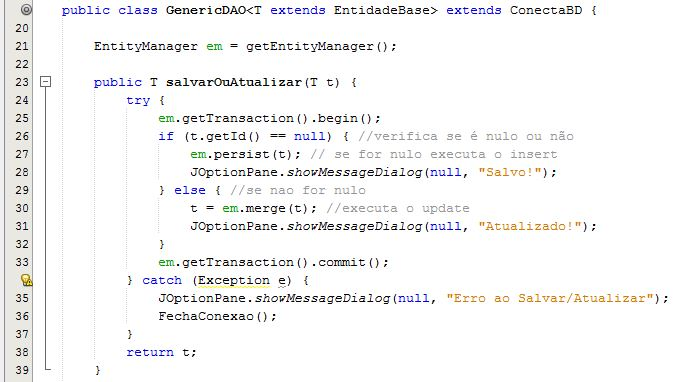
\includegraphics[width=12cm]{imagens/codigo/TrechoGenericDao}
\fonte{Autor próprio}
\label{fig:Dao Genérico}
\end{figure}
   
   Os métodos das classes DAO são responsáveis por realizar consultas personalizadas de cada entidade, como consultar por id ou nome. Abaixo um método de consulta personalizadas:
   
 \begin{figure}[H]
\centering
\caption{Código - Classe DAO}
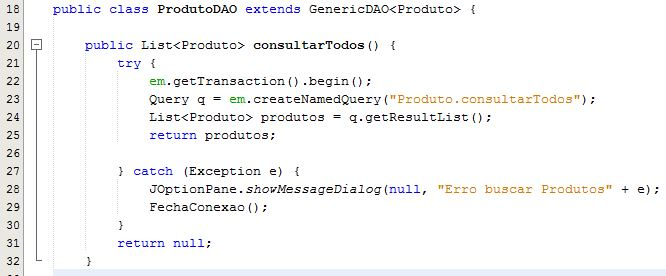
\includegraphics[width=13cm]{imagens/codigo/TrechoDao}
\fonte{Autor próprio}
\label{fig:Classe DAO}
\end{figure}
    
    \subsection{JasperReport}
    Abaixo o método de geração de relatórios em java utilizando o JasperReport:
    
\begin{figure}[h]
\centering
\caption{Código - Geração de relatório}
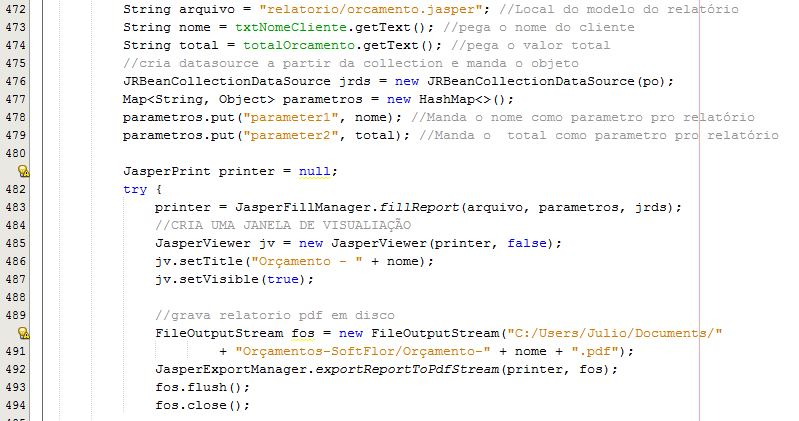
\includegraphics[width=15cm]{imagens/codigo/TrechoJasper}
\fonte{Autor próprio}
\label{fig:Método Relatório}
\end{figure}
    
    \subsection{Controle de acesso}
    
    Para garantir que somente usuários cadastrados pelo administrador tenham acesso ao sistema, foi implementado uma tela de Login onde o usuário deve informar os dados de acesso (Usuário e senha). O sistema verifica as informações e libera ou recusa o acesso. Como \textit{default} o sistema virá com super usuário cadastrado (Administrador), somente este super usuário pode gerenciar os outros usuários cadastrados, exceto alteração de senha. O método que realiza a liberação do aceso pode ser visto a seguir:
    
\begin{figure}[h]
\centering
\caption{Código - Controle de acesso}
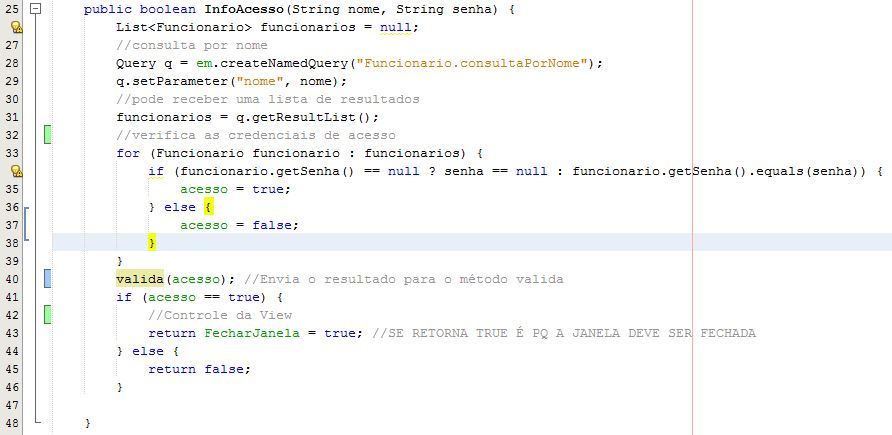
\includegraphics[width=15cm]{imagens/codigo/TrechoAcesso}
\fonte{Autor próprio}
\label{fig:Controle de acesso}
\end{figure}
    
     \subsection{Validação dos dados}
     É comum o usuário enviar dados inesperados como entradas para o sistema, por isso, devemos garantir que os dados informados sejam compatíveis com os esperados. Através deste princípio foram desenvolvidos métodos de verificação dos dados na camada de visualização do sistema.
     
    
    
\section{Telas do sistema}
A seguir são mostradas algumas telas de utilização do sistema SOFTFLOR. Como a tela de entrada do funcionário, tela principal do sistema, lista de fornecedores, cadastro de produtos e clientes, elaboração e geração de orçamentos.
\subsection{Login}
A Figura \ref{fig:Tela-de-Login} mostra a tela de entrada do funcionário. Para entrar no sistema, o funcionário precisa se identificar, informando seu nome de usuário e sua senha. Após informar estes dados, o sistema irá fazer a verificação e autorização de entrada do funcionário.
\begin{figure}[H]
\centering
\caption{Tela de login}
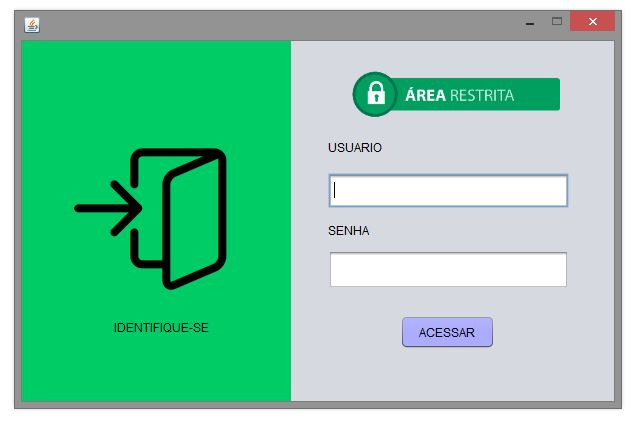
\includegraphics[width=11cm]{imagens/telas/Login}
\fonte{Autor próprio}
\label{fig:Tela-de-Login}
\end{figure}
      
      
\subsection{Principal}
A tela principal do sistema pode ser vista na Figura \ref{fig:Tela-principal}. O funcionário tem a facilidade de acessar algumas funcionalidades através do menu rápido, como a lista de clientes, fornecedores, produtos e geração de orçamentos. Outras funcionalidades podem ser acessadas através do menu superior da tela principal.

\begin{figure}[H]
\centering
\caption{Tela principal}
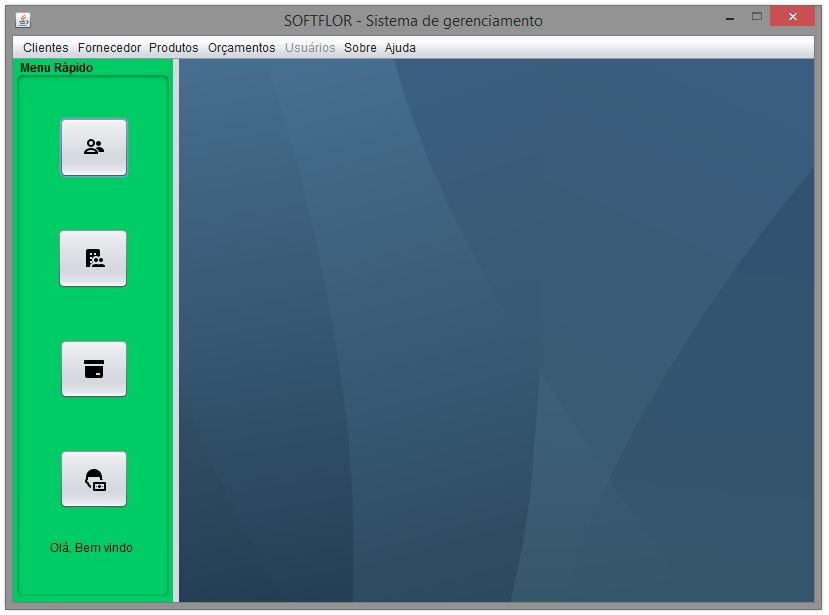
\includegraphics[width=12cm]{imagens/telas/Principal}
\fonte{Autor próprio}
\label{fig:Tela-principal}
\end{figure}
       
\subsection{Lista de fornecedores}
A Figura \ref{fig:Lista-de-fornecedores} mostra a tela de listagem de fornecedores, é possível editar informações, cadastrar um novo fornecedor, ver produtos associados ou excluir um fornecedor.
\begin{figure}[H]
\centering
\caption{Lista de fornecedores}
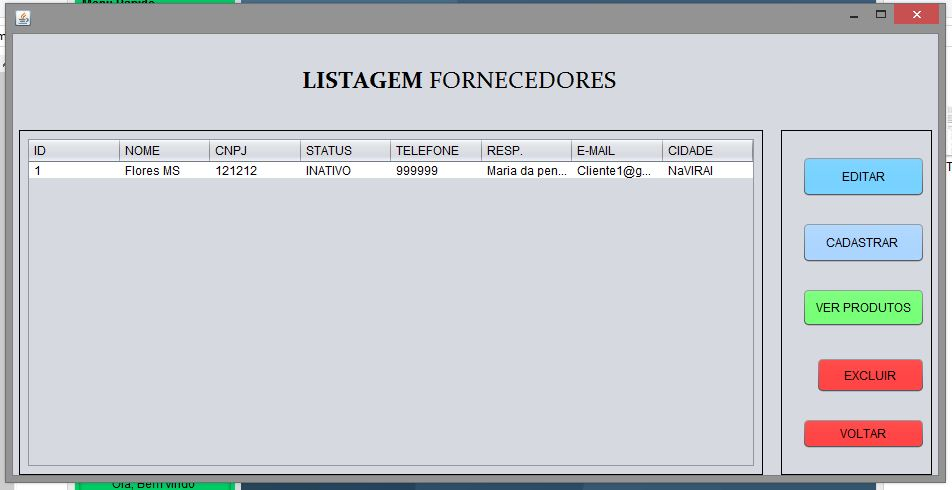
\includegraphics[width=14cm]{imagens/telas/ListaFornecedor}
\fonte{Autor próprio}
\label{fig:Lista-de-fornecedores}
\end{figure}
       
\subsection{Lista de produtos}
%A Figura \ref{fig:Lista-de-produtos} mostra a tela de produtos cadastrados no banco de dados. As informações mostradas contém o código, nome, quantidade atual no estoque, preço de compra, preço de venda, quantidade mínimo que produto pode ter no estoque e a unidade de medida referente ao produto. Além disso, o funcionário pode cadastrar um novo produto ou editar as informações de um produto já cadastrado no sistema.

A Figura \ref{fig:Lista-de-produtos} mostra a tela de produtos cadastrados. Contém as informações referente aos produtos. O funcionário pode cadastrar, editar ou excluir produtos.
\begin{figure}[H]
\centering
\caption{Lista de produtos}
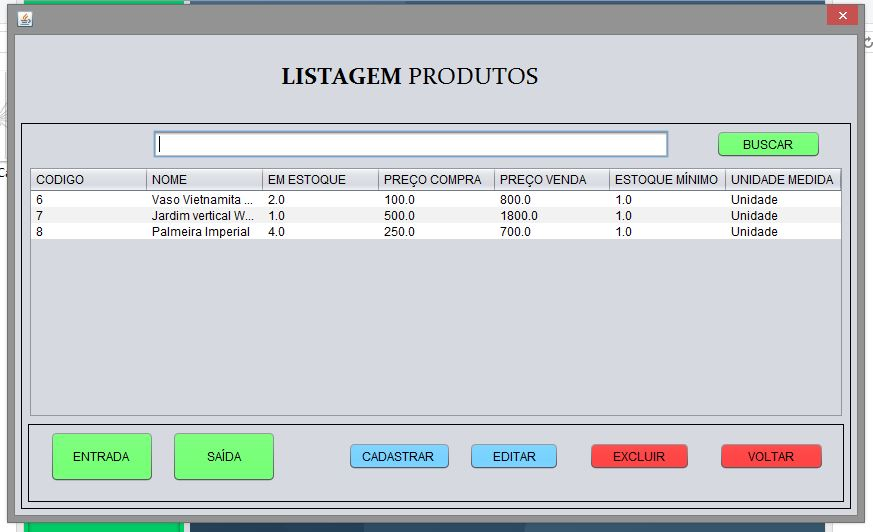
\includegraphics[width=14cm]{imagens/telas/ListaProdutos}
\fonte{Autor próprio}
\label{fig:Lista-de-produtos}
\end{figure}
        
        
\subsection{Lista de clientes}

A Figura \ref{fig:Lista de clientes} exibe a tela de clientes cadastrados no sistema. 
        
 \begin{figure}[H]
\centering
\caption{Lista de clientes}
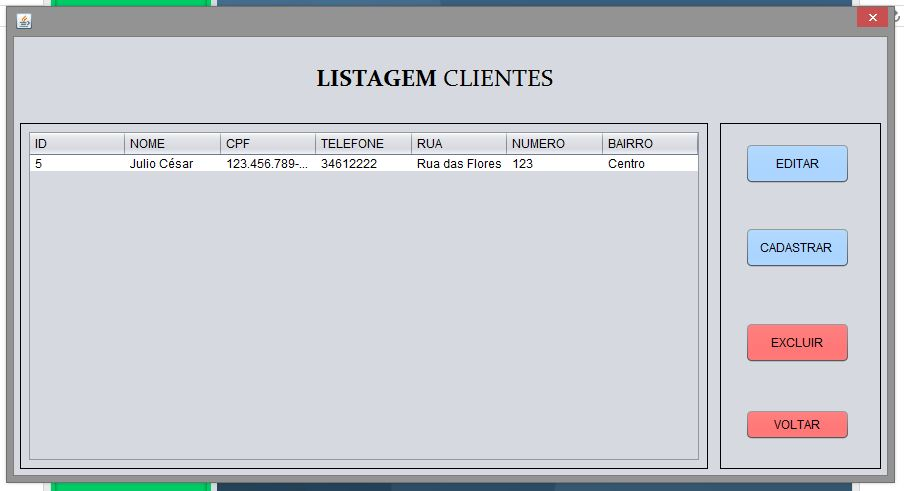
\includegraphics[width=14cm]{imagens/telas/ListaCliente}
\fonte{Autor próprio}
\label{fig:Lista de clientes}
\end{figure}
        
Nesta tela, exibirá informações pessoais de cada cliente, além de dados de contato e endereço. O Funcionário poderá, ainda, editar ou excluir um cliente, além de cadastrar um novo cliente no banco de dados do sistema.    
        
\subsection{Elaboração de orçamentos}
A Figura \ref{fig:Geração de orçamento} exibe a tela onde são gerados os orçamentos. Primeiramente o funcionário  busca pelo cliente cadastrado no sistema. Em seguida, são inseridos os produtos desejados no orçamento, que gera automaticamente o custo total dos produtos. A qualquer momento o funcionário poderá excluir um produto da lista. Por fim o funcionário poderá salvar ou gerar um orçamento elaborado.

\begin{figure}[H]
\centering
\caption{Geração de Orçamentos}
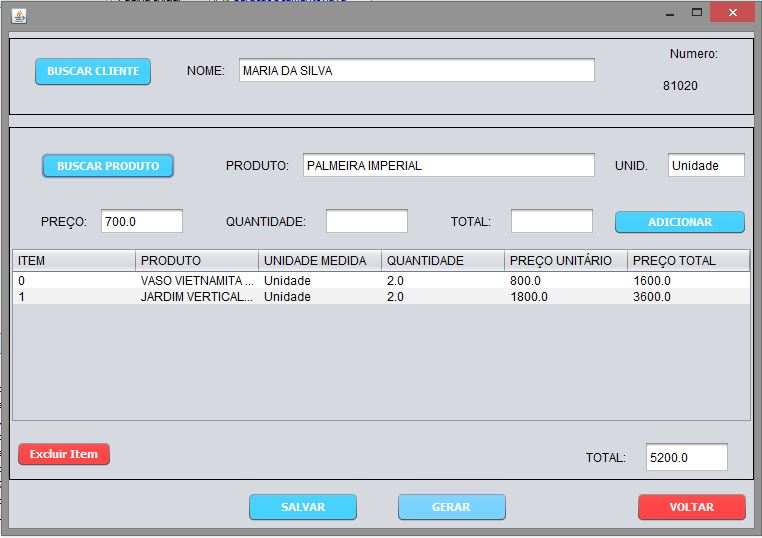
\includegraphics[width=14cm]{imagens/telas/GeraOrcamento}
\fonte{Autor próprio}
\label{fig:Geração de orçamento}
\end{figure}      

\subsection{Orçamento gerado}
A figura á seguir \ref{fig:Orçamento Gerado} apresenta um orçamento gerado através da tela \ref{fig:Geração de orçamento}. Nesta tela o funcionário poderá salvar e imprimir o orçamento. Também são apresentados informações quanto ao valor total do orçamento e a data de geração.
\begin{figure}[H]
\centering
\caption{Orçamento gerado}
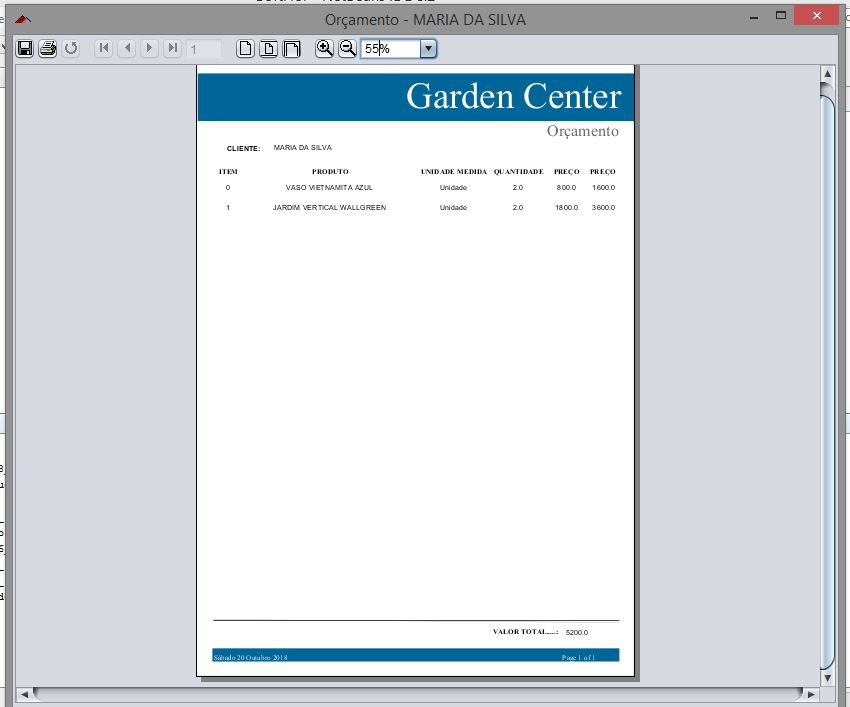
\includegraphics[width=15cm]{imagens/telas/OrcamentoGerado}
\fonte{Autor próprio}
\label{fig:Orçamento Gerado}
  
\end{figure}  
      
\section{Testes de software}  

A fase de teste é muito importante no desenvolvimento de software pois é esta fase que busca constatar se sistema atende ou não os requisitos levantados na ciclo inicial de desenvolvimento.
Em engenharia de software existem diversas técnicas que podem ser utilizadas em vários momentos durante o processo de desenvolvimento de software e que visam atender duas metas distintas, sendo: demonstrar que o sistema atende aos requisitos levantados e detectar, localizar e reparar falhas ou comportamentos não desejados. No desenvolvimento deste projeto utilizaremos a técnica de teste estrutural e técnica de teste funcional. 

\subsection{Teste de caixa branca}

Este tipo de teste é desenvolvido analisando-se o código fonte e elaborando-se casos de teste que cubram todas as possibilidades
do componente de software \cite{neto2007introduccao}.
Esta técnicas foi utilizada durante todo o processo de desenvolvimento de software. A cada método criado e cada objeto instanciado foram feitos pequenos testes nos códigos buscando detectar falhas. As falhas detectadas foram corrigidas, entretanto, o código deve continuar em constantes testes,sobretudo quando novas funcionalidades ou ferramentas forem inseridas no sistema. 
      

\subsection{Teste de caixa preta}
O teste de caixa preta foi implementado ao final do projeto, diferente do teste de caixa branca não deve ser realizado em contato com o código fonte do sistema, ou seja, são realizados testes simulando a usabilidade do usuário. 

 Dados de entrada são fornecidos, o teste é executado e o resultado obtido é comparado a um resultado esperado previamente conhecido.
Haverá sucesso no teste se o resultado obtido for igual ao resultado esperado \cite{neto2007introduccao}.
    As tabelas a seguir apresentam alguns testes realizados no sistema e os resultados obtidos.

% Please add the following required packages to your document preamble:
% \usepackage{booktabs}
\begin{table}[H]
\caption{Resultado de teste - Cadastrar produto}
\label{tab:testeCadProduto}
\resizebox{\textwidth}{!}{\begin{tabular}{lll}
\hline
\multicolumn{3}{c}{\textbf{Testes - Manter Produto}}                                                                 \\ \hline
\textbf{Teste}                              & \textbf{Resultado}                                                    & \textbf{Situação}  \\ \hline
Cadastro de produto sem fornecedor & Erro: Produto cadastrado                                     & Corrigido \\ \hline
Cadastro com campo vazio           & \begin{tabular}[l]{@{}l@{}}Produto não é cadastrado.\\Não emite mensagem de erro.\end{tabular}          & Pendente  \\ \hline
Cadastro produtos idênticos        & \begin{tabular}[l]{@{}l@{}}O mesmo produto pode ser cadastrado\\para o mesmo fornecedor.\end{tabular} & Pendente  \\ \hline
Excluir produto da lista           & Item excluído do banco e da tabela                           & Cumprido  \\ \hline
Editar produtos da lista           & Item editado e tabela atualizada                             & Cumprido  \\ \hline
\end{tabular}}
\fonte{Autor próprio.}
\end{table}


\subsection{Teste de compatibilidade}
Atualmente existente diversos sistemas operacionais que funcionam nos mais variados tipos de hardware. Para garantir o bom funcionamento do sistema é importante realizar o maior numero de testes possíveis afim de evitar possíveis problemas de incompatibilidade. Na tabela abaixo alguns testes realizados:

% Please add the following required packages to your document preamble:
% \usepackage{booktabs}
\begin{table}[H]
\centering
\caption{Teste compatibilidade}
\label{tab:testeCompatibilidade}
\resizebox{\textwidth}{!}{\begin{tabular}{ccccc}
\hline
\multicolumn{5}{c}{\textbf{Teste - Compatibilidade}}                                   \\ \hline
\textbf{Sistema operacional} & \textbf{Memória RAM} & \textbf{Processador}   & \textbf{Disco Rígido} & \textbf{Status}       \\ \hline
Windows 8.1         & 8 GB        & Intel Core i5 & 500 GB       & Satisfatório \\ \hline
Windows 7           & -           & -             & -            & Pendente     \\ \hline
Windows 10          & -           & -             & -            & Pendente     \\ \hline
Ubuntu              & -           & -             & -            & Pendente     \\ \hline
\end{tabular}}
\fonte{Autor próprio.}
\end{table}

\subsection{Teste de segurança}
Os testes de segurança são realizados afim de evitar acesso indesejado ao sistema e seu banco de dados. A seguir o resultado dos testes realizados: 

% Please add the following required packages to your document preamble:
% \usepackage{booktabs}
\begin{table}[H]
\centering
\caption{Resultado de teste - Segurança}
\label{tab:testeSegurança}
\resizebox{\textwidth}{!}{\begin{tabular}{ccc}
\hline
\multicolumn{3}{c}{\textbf{Teste - Segurança}} \\ \hline
\textbf{Teste} & \textbf{Resultado} & \textbf{Situação}     \\ \hline
Página de login & \begin{tabular}[c]{@{}c@{}}Acesso é restrito a usuários cadastrados.\\ Exibe mensagens aos usuários\end{tabular}      & Satisfatório \\ \hline
Exclusão de itens & Solicita confirmação de exclusão & Satisfatório \\ \hline
Salvamento de arquivos falhos & \begin{tabular}[c]{@{}c@{}}Rollback é realizado quando ocorre uma\\ falha na persistência de objetos\end{tabular} & Satisfatório \\ \hline
Acesso a lista de usuários & Não é possível obter lista de usuários & Pendente     \\ \hline
Criptografia de senhas & Não existe método de criptografia & Pendente     \\ \hline
\end{tabular}}
\fonte{Autor próprio.}
\end{table}

\subsection{Teste de sistema}
Consiste em realizar testes utilizando o sistema em sua versão de \textit{release}, ou seja, pronto para enviar ao usuário. Deve testar as principais atividades que serão realizadas e documentar os resultados.

% Please add the following required packages to your document preamble:
% \usepackage{booktabs}
\begin{table}[H]
\caption{Resultado de teste - Sistema}
\label{tab:testeSistema}
\centering
\begin{tabular}{ccc}
\hline
\multicolumn{3}{c}{\textbf{Testes do sistema}} \\ \hline
\textbf{Teste} & \textbf{Resultado} & \textbf{Situação}     \\ \hline 
Acesso ao sistema & Primeiro acesso é lento & Razoável     \\ \hline
Teste das ações dos botões & \begin{tabular}[c]{@{}c@{}}Todas as ações ocorreram\\ dentro do esperado\end{tabular}           & Satisfatório \\ \hline
Elaboração do orçamento & Elaborado com sucesso & Satisfatório \\ \hline
Geração do orçamento & Tela de visualização com lentidão & Razoável     \\ \hline
\begin{tabular}[c]{@{}c@{}}Cadastro de produto a\\ partir da tela de listagem\end{tabular} & \begin{tabular}[c]{@{}c@{}}Não retorna a tela de listagem\\ ao realizar a operação\end{tabular} & Satisfatório \\ \hline
\end{tabular}
\fonte{Autor próprio.}
\end{table}

\section{Implantação do sistema}

O sistema atenderá as demandas do Garden Center do espaço Café com Flores. Neste espaço, além do garden, funciona o escritório Torre Forte Engenharia Elétrica e Agronômica onde são desenvolvidos os projetos de paisagismo que utilizam os produtos que serão armazenados neste sistema. A instalação do \textit{software} será em computador \textit{Desktop} equipado com 4GB de memória RAM, processador Intel Core i3 e sistema de operacional \textit{Windows} 7 64 bits.